\documentclass[a4paper,11pt]{article}
\usepackage{graphicx}
\usepackage{booktabs}
\usepackage{tabularx}
\usepackage{url}
\usepackage{pdfpages}
\usepackage{epstopdf}
\usepackage{multicol}

\graphicspath{ {images_eps/} }

%
% Do not change
\textheight = 220mm
\textwidth  = 150mm
\topmargin  = 10mm
\oddsidemargin  = 5.0mm
\evensidemargin = 5.0mm
\unitlength = 1mm

\usepackage[utf8]{inputenc}
\usepackage[T1]{fontenc}
\usepackage[swedish]{babel}

\begin{document}
%
% Do not change
\let\rempage=\thepage
{
\renewcommand{\thepage}{\relax}
\begin{picture}(44,0)(15,10)
% \special{psfile=mahlogo-name.eps}

\includegraphics[scale=1]{mahlogo-name.eps}
\end{picture}

\vspace*{-30mm}
\hfill\begin{minipage}[t]{16em}\large
Fakulteten för teknik och samhälle\\
Datavetenskap
\end{minipage}

\vspace*{45mm}
\begin{center}
{\bf\large
Examensarbete 

\small
15 högskolepoäng, grundnivå
}

\vspace*{25mm}
\LARGE
%
% Put your title here
LEAP: Automatiserad bedömning av programmeringsuppgifter

\vspace*{8mm}
\large
%
% Translated title 
LEAP: Automatic assessment of programming assignments

\vspace*{12mm}
\Large
%
% Author names
Felix Alhbin\\
Mattias Pernhult

\vspace*{30mm}
\large
%
% Picture if you want
\end{center}

\vfill
\hspace*{-10mm}%
\begin{minipage}[t]{20em}
%
% Fill in correct data for you
Examen: Kandidatexamen 180~hp
\\
Huvudområde: Datavetenskap
%
% Huvudområden är:
% Affärssystem
% Data och informationsvetenskap (IA och IS)
% Datavetenskap (Övriga)
\\
Program: Systemutvecklare
\\
Datum för slutseminarium: 2016-05-30
\end{minipage}
%
\hfill
%
\begin{minipage}[t]{15,5em}
%
% Fill in supervisor and second reader
Handledare: Ulrik Eklund
\\
Andrabedömare: Magnus Krampell
\end{minipage}

\newpage

\mbox{}

\newpage

\section*{Sammanfattning}

Antal studenter i programmeringskurser på universitet och högskolor ökar kraftigt och kräver mycket resurser vilket gör kurserna nästintill omöjliga att bedriva utan att öka antalet lärare. Genom att introducera automatisering i dessa kurser, speciellt vid bedömning, är det möjligt att upprätthålla kvalitén i dessa kurser. Därav är syftet med denna studie att konstruera, implementera och utvärdera ett bedömningssystem för att ta reda på för- och nackdelar med användningen av bedömningssystem i programmeringskurser. Resultatet från studien visar att fördelarna med ett bedömningssystem är direkt återkoppling, dess tillgänglighet och dess förmåga att verifiera korrektheten av studenters program bättre än vad en lärare kan. Resultatet visar att nackdelarna med ett bedömningssystem är dess ökad krav på välutformade uppgifter och testfall samt systemets svårighet att bedöma kvalitativa aspekter i studenters program.

\newpage

\mbox{}

\newpage

\section*{Abstract}

Number of students in programming courses at universities is increasing rapidly and requires a lot of resources which makes the courses almost impossible to conduct without increasing the number of teachers. By introducing automation in these courses, especially in the assessment part, it is possible to maintain the quality of these courses. Hence, the aim of this study is to design, implement and evaluate an assessment system to find out the benefits and drawbacks of the use of a assessment systems in programming courses. The results of the study shows that the benefits of an assessment system is direct feedback, its availability and its ability to verify the accuracy of students programs better than a teacher. The result shows that the drawbacks of an assessment system is its increased effort of designing well-designed tasks and test cases, as well as the systems inability to assess the qualitative aspects of the students programs.

\begin{description}
    \item[Keywords] Automated assessment system, test cases, feedback, computer programming courses, quiz, LEAP, sandbox
\end{description}

\newpage

\section*{Ordlista}
\begin{description}
    \item [Docker] En containerbaserad virtualiserings plattform
    \item [Docker-container] En Docker-container är en lättviktig isolerad process som körs ovanpå hostens operativssystem
    \item [Git] Ett distribuerat versionshanteringssystem
    \item [Versionshanteringssystem] Ett verktyg som gör det möjligt att lagra, återskapa och spåra ändringar i dokument och källkodsfiler
    \item [REST-API] Ett gränssnitt vilket mjukvarusystem kommunicerar via som följer IT arkitekturen Representational State Transfer (REST)
    \item [NoSQL] Databashanterare som tillhandahåller lagring och hämtning av data som ej behöver vara tabulär.
    \item [OAuth 2.0] En öppen standard för autentisering som används för att autentisera personer genom tredjepartstjänster
    \item [Testfall] Strukturerat testunderlag som beskriver hur en funktion eller egenskap ska testas. Innehåller bland annat teststeg och förväntat resultat
    \item [Enhetstestning] En mjukvarutestningsmetod som används för att verifiera att källkoden fungerar som den är specificerad att göra
    \item [JUnit] Ett ramverk för enhetstestning av programmeringsspråket Java
    \item [Exekveringsmiljö] Program, filer och rutiner som, förutom operativsystemet, behövs för att man ska kunna köra ett visst program
\end{description}


\newpage

\mbox{}

\newpage
\tableofcontents
\newpage
\ifodd\value{page}\else\mbox{}\newpage\fi
\setcounter{page}{1}
\renewcommand{\thepage}{\rempage}

\section{Inledning}

\subsection{Bakgrund}\label{Bakgrund}

Ett sätt att lära sig att programmera är genom introduktionskurser på universitetet. I sådana kurser ges studenter olika uppgifter som kan hjälpa dem att bli bekanta med moderna programmeringsspråk, lära sig viktiga verktyg och få insikter om hur systemutveckling bedrivs \cite{douce_11}. Utvärdering och bedömning av dessa programmeringsuppgifter utförs vanligtvis manuellt av lärare och labbhandledare. När kurser utförs på detta traditionella sätt och de innehåller ett högt antal studenter skapar det tunga och tidskrävande uppgifter för lärare och övningsassistenter vilket tär på universitetets resurser. Det innebär även att återkopplingen till studenterna fördröjs vilket har en negativ påverkan på deras utveckling jämfört med direkt återkoppling \cite{japanerna_1}. Eftersom potentiella lösningar till mindre programmeringsuppgifter är av likartad karaktär kan utvärdering och bedömning automatiseras genom automatiserade bedömningssystem. Därav kan lärares resurser användas på ett mer effektivt sätt och på så vis förbättra kvalitén i kursens andra moment samtidigt som det ger en objektiv bedömning och direkt återkoppling till studenterna \cite{douce_11} \cite{hollingsworth_2} \cite{higgins_3}. Automatiserade bedömningssystem för programmeringsuppgifter nämns redan första gången 1960 av Hollingsworth \cite{hollingsworth_2}. Studenterna använde sig av hålkort med program skrivna i assembly som de skickade in för bedömning. Sedan dess har automatiserade bedömningssystem vidareutvecklats.

\subsection{Relaterat arbete}

Daly och Horgan \cite{roboprof_4} presenterar i sin artikel hur de utvecklade det automatiserade lärningssystemet RoboProf \cite{roboprof_4}. I artikeln utförde de även en studie där de testade att använda RoboProf i en introduktionskurs för programmering. Resultaten från studien visar att de studenter som utförde kursen på ett traditionellt vis presterade betydligt sämre än de studenter som använde RoboProf. Vidare presenterar författarna även en lösning för plagieringsproblemet vilket bygger på en idé av Plauger \cite{plaguer_5}.

Rößling och Hartte tar i sin artikel \cite{webtasks} upp en webb-baserat lärningsplattform som de kallar för WebTasks som bedömer programmeringsuppgifter för Java programmering. Det intressanta med WebTasks är att när en students lösning accepteras av WebTasks sparas lösningen och den görs tillgänglig för andra studenter som även de har fått sina lösningar accepterade. Därmed finns det möjlighet för granskning och diskussion av de olika lösningarna och därav kanske studenterna kan komma fram till alternativa eller effektivare lösningar.

I artikel \cite{edwards_15} presenterar Edwards och Pérez-Quiñones sina erfarenheter av att använda testdriven utveckling med Web-CAT \cite{edwards_15}. Web-CAT är unikt bland automatiserade bedömningssystem eftersom det bedömer hur bra studenterna testar sin egen kod istället för att studenternas kod testas gentemot fördefinierade testfall \cite{edwards_15}.

Higgins m. fl. \cite{higgins_3} påpekar i sin studie om det automatiserade bedömningssystemet CourseMarker \cite{higgins_coursemarker_12} att studenter ofta vill ha detaljerad information om vilken del av deras kod som inte godkändes. Författarna hävdar dock att alltför detaljerad information i återkopplingen kan ha negativ påverkan på studenters resultat. CourseMarker löser problemet genom att låta läraren själv ange hur detaljerad återkopplingen till studenten ska vara \cite{higgins_3} \cite{caiza_7} \cite{douce_11}.

En alternativ lösning presenteras av Reek som begränsar antalet försök en student har på sig att genomföra en uppgift. Detta för att tvinga studenterna att tänka över sina lösningar mer noggrant innan de lämnar in dem \cite{reek_6}. Denna lösning presenteras även av Ihantola m. fl. \cite{ihantola}.

Caiza och Del Alamo tar även de upp problem kring återkoppling till studenter \cite{caiza_7}. De nämner \textit{trial and error}-problemet vilket betyder att studenter prövar sig fram genom att göra mindre förändringar i deras program istället för att reflektera över vad problemet beror på. Författarna påstår att de inte upplevt \textit{trial and error}-beteendet bland de medverkande studenterna.

Ihantola m. fl. \cite{ihantola} lyfter fram olika lösningar för att förhindra \textit{trial and error}-beteendet.  En alternativ lösning som de presenterar är att begränsa mängden återkoppling till studenten. Dock kan detta frambringa förvirring hos studenten eftersom studenten inte förstår varför programmet bedömdes som inkorrekt [26]. Vidare nämner författarna en lösning där studenten får en tidsbestraffning vid ett misslyckande, de påpekar även att tidsbestraffningen kan öka exponentiellt.
De presenterar även en lösning där studenten får en slumpmässigt utvald uppgift vid varje nytt försök vilket förhindrar \textit{trial and error} beteendet. 

Hollingsworth påpekar att studenters program kan innehålla skadlig kod vilket kan förstöra bedömningssystemet, de utgör därmed ett hot mot systemet \cite{hollingsworth_2}. Detta problem adresseras av artiklarna \cite{spacek_13} \cite{cs50_8} \cite{ihantola} där författarna presenterar två alternativa lösningar som bygger på grundtanken att kompilera och exekvera studenternas program i en säker miljö för att skydda bedömningssystemet. I artikeln \cite{cs50_8} presenterar Malan bedömningssystemet CS-50 vilket utvecklades som en del av en internetbaserad kurs vid Harvard Universitetet. För att säkert kompilera och exekvera opålitlig kod använder CS-50 SELinux \cite{selinux} och PAM begränsningar \cite{pambegransningar}. Špaček m. fl. \cite{spacek_13} hävdar i sin studie att flertalet av dagens bedömningssystem saknar stöd för exekvering av opålitliga program i en säker miljö. Författarna har i sin lösning valt att använda den virtuella containerbaserade plattformen Docker \cite{docker} för att kompilera och exekvera studenternas program. APAC verifierar studenternas program genom att analysera och validera programmets utdata.

\subsection{LEAP}

Under vår litteraturstudie av liknande bedömningssystem har vi observerat att avsaknaden av exekvering i säker miljö är vanligt förekommande i flertalet system [Review] \cite{roboprof_4} [CourseMarker]. Denna observation stöds även av Spacek m. fl. \cite{spacek_13}. Vi har även observerat att majoriteten av bedömningssystemen verifierar studenternas program genom att analysera och validera programmets utdata gentemot utdatan från ett korrekt implementerat program [Review] [RIT]. Våra observationer låg till grund för LEAP vilket är den prototyp som implementerades för att kunna besvara frågeställningen. Namnet LEAP är en förkortning av \textit{LEarning and Assessment of Programming}. LEAP använder sig av testfall som skapas av lärare för att bedöma studenters lösningar och för att garantera att studenternas program exekverar i en säker miljö använder sig LEAP av Docker-containrar.

LEAP bedömer studentens lösning genom att köra fördefinierade testfall i form av enhetstester mot studentens kod, om samtliga testfall passeras kommer LEAP meddela studenten att lösningen är godkänd. Om något testfall misslyckas kommer LEAP meddela studenten att lösningen inte är godkänd och att studenten får försöka igen, LEAP meddelar även vad det vad som inte godkändes. LEAP beskrivs mer utförligt under avsnitt \ref{LEAP}.


\subsection{Syfte}

Studien ämnar att konstruera, implementera och utvärdera ett bedömningssystem som är tänkt att användas i programmeringskurser som bedrivs på Malmö Högskola. Syftet är dels att undersöka vilka för- och nackdelarna är av att använda ett bedömningssystem i programmeringskurser och dels att undersöka vilka fördelar respektive nackdelar som ett bedömningssystem har vid bedömning av programmeringsuppgifter och dels undersöka hur bedömningssystem kan användas i programmeringskurser.

\subsection{Frågeställning}

Studien avser ge svar på följande frågor:

\begin{enumerate}
\item
Vilka är för- och nackdelarna av att använda ett bedömningssystem av den här typen i programmeringskurser?
\item
Hur kan ett bedömningssystem av den här typen användas i programmeringskurser?
\end{enumerate}

\subsection{Avgränsning}

Vi har under litteraturstudien identifierat att det finns olika aspekter inom bedömning av programmeringsuppgifter [KÄLLA] som bedömning av funktionalitet vilket innebär att lösningens korrekthet verifieras och även bedömning av lösningens design- och implementationsval vilket är en bedömning av lösningens kvalité.
\\
\\
LEAP kommer enbart att bedöma lösningens korrekthet och inte göra någon form av bedömning eller analys av lösningens kvalité utan enbart verifiera lösningens funktionalitet. Därmed är tanken att LEAP inte ska ersätta hela bedömningsprocessen utan istället fungera som ett stöd för lärare i deras bedömningsprocess och eventuellt minska de resurser som lärare lägger på att bedöma ofullständiga lösningar.
\\
\\
De respondenter och testpersoner som deltar i studien för att besvara frågeställningen är lärare och studenter på Malmö Högskola inom institutionen Datavetenskap.

\newpage
\section{Metod}\label{Metod}

Följande avsnitt beskriver den metodik som valts för utförandet av studien. I avsnitt \ref{Nunamakers metod} presenterar vi Nunamakers metod och hur de två andra metoderna, intervjuer och kontrollerade experiment, relaterar till Nunamakers metod vilket presenteras visuellt i Figur \ref{fig:metod_visual}. Intervjuerna används som underlag för att definiera systemkrav och experimenten utförs för att utvärdera LEAP. Förtydligande av intervjuerna och experimenten presenteras i avsnitt \ref{Intervjuer} respektive avsnitt \ref{Experiment}.
\\
\\
Eftersom studiens syfte är att konstruera, implementera och utvärdera en systemartefakt valdes en metodik som presenteras av Nunamaker m. fl. \cite{nunamaker} eftersom det är en erkänd och välbeprövad process för forskning inom informationssystem. Författarna definierar en iterativ femstegsprocess för hur sådan forskning bör bedrivas vilken innefattar att: \textit{(1) konstruera ett konceptuellt ramverk} \textit{(2) utveckla en systemarkitektur} \textit{(3) konstruera och analysera systemet} \textit{(4) implementera systemet} och \textit{(5) utvärdera systemet}. 
\\
\\
För att ytterligare säkerställa studiens kvalité följer den de sju riktlinjer för forskning inom informationssystem definierade av Hevner m.fl. \cite{hevner}:
\begin{description}
    \item [Riktlinje 1]
    Design as an Artifact
    \begin{itemize}
    \item [--] Riktlinje 1 innebär enligt Hevner m.fl att forskning inom informationssystem måste producera en artefakt. I avsnitt \ref{LEAP} presenteras artefakten.
    \end{itemize}
    \item [Riktlinje 2]
    Problem Relevance
     \begin{itemize}
    \item [--] Målet med forskning inom informationssystem är att utveckla teknologibaserade lösningar på viktiga och relevanta affärsproblem. Studiens relevans presenteras i avsnitt \ref{Bakgrund}
    \end{itemize}
    \item [Riktlinje 3]
    Design Evaluation
     \begin{itemize}
    \item [--] En artefakts användbarhet, kvalité och effektivitet måste demonstreras via strikta utvärderingsmetoder. Utvärdering av artefakten ingår i steg 5 i Nunamakers process och beskrivningen av utförandet presenteras under avsnitt \ref{Experiment} och resultatet under avsnitt \ref{experiment} 
    \end{itemize}
    \item [Riktlinje 4]
    Research Contributions
     \begin{itemize}
    \item [--] Forskning inom informationssystem måste tillhandahålla tydliga och verifierbara resultat. Diskussion kring resultatens validitet finns under avsnitt \ref{TODO}
    \end{itemize}
    \item [Riktlinje 5]
    Research Rigor
     \begin{itemize}
    \item [--] Forskning inom informationssystem måste använda sig av rigorösa metoder vid både utveckling och utvärdering av artefakten. I avsnitt \ref{Metod} presenteras studiens metodval.
    \end{itemize}
    \item [Riktlinje 6]
    Design as a Search Process
     \begin{itemize}
    \item [--] Riktlinje 6 innebär i praktiken att iterera steg 3-5 i Nunamakers process, se figur \ref{fig:metod_visual}. 
    \end{itemize}
    \item [Riktlinje 7]
    Communication of Research
     \begin{itemize}
    \item [--] Med riktlinje 7 menar Hevner m.fl att forskning inom informationssystem måste presenteras effektivt till både teknikkunnig såväl som icke-teknikkunnig publik. Uppsatsen i sig är vårt sätt att presentera studien. 
    \end{itemize}
\end{description}

\subsection{Nunamakers metod}\label{Nunamakers metod}

\begin{figure}[ht!]
\centering
\includegraphics[scale=0.4]{metod_image2.eps}
\caption{Visuell presentation av våra metoder och deras relation}
\label{fig:metod_visual}
\end{figure}

Steg 1 i Nunamakers metod är att konstruera ett konceptuellt ramverk vilket innebär att definiera relevanta systemkrav. För att identifiera och definiera dessa genomför vi en litteraturstudie av liknande system och intervjuar tre lärare vid Malmö högskola. Vi väljer ut tre lärare som alla har lång, dokumenterad erfarenhet av att lära ut programmering till högskolestudenter i introduktionskurser. Valet av intervjupersoner anser vi vara befogat eftersom personerna i fråga är representativa för den huvudsakliga målgruppen och verksamma inom den miljö som systemet ska tillämpas. Därav får vi djupare förståelse för hur lärarna bedriver programmeringskurser och hur lärarna tänker kring bedömning av programmeringsuppgifter. Denna förståelse och information som vi samlar in från intervjuerna med lärarna hjälper oss att definiera krav för systemet.
Anledningen till att vi inte väljer en kvantitativ undersökningsmetod som exempelvis enkäter med fördefinierade svar beror på att de endast ger en ytlig förståelse i ämnet till skillnad från intervjuer \cite{seminarieboken}. Vid intervjuer finns det även utrymme för att ställa följdfrågor till respondenten samt att det går att förtydliga frågorna vid eventuella missuppfattningar, något som inte är möjligt vid fördefinierade enkätundersökningar \cite{seminarieboken}. Informationen som vi samlar in från litteraturstudien används för att urskilja de befintliga systemen. Därigenom identifieras funktioner som vi anser saknas i dessa system vilket gör att vi, tillsammans med informationen från intervjuerna, kan definiera krav som systemets ska uppfylla.
\\
\\
Enligt Nunamaker m. fl. innefattar steg 2 att definiera systemets komponenter och att definiera förhållandet mellan komponenterna samt att identifiera och definiera systemets funktionalitet \cite{nunamaker}. Den insamlade informationen från steg 1 analyseras och sammanställs till systemkrav och systemfunktioner. De används sedan för att definiera komponenter och funktioner för systemet\footnote{Resultatet från detta steg finns i avsnitt \ref{systemfunktioner}}. Nunamaker m.fl. påpekar betydelsen av att definiera mätbara funktioner för systemet eftersom det underlättar vid systemutvärderingen \cite{nunamaker}.
\\
\\
I det tredje steget, konstruera och analysera systemet, är syftet att vi identifierar möjliga lösningar, tekniker och språk för att implementera systemet i kommande steg \cite{nunamaker}. Möjliga lösningar konstrueras och analyseras innan vi slutligen väljer det bästa alternativet att gå vidare med och implementera\footnote{Resultatet från detta steg finns i avsnitt \ref{systemkomponenter}}.
\\
\\
Tanken med det fjärde steget är att implementera en prototyp som utvärderas i kommande steg. Prototypen beskrivs under avsnittet \ref{LEAP}. Prototypen ger insikter angående konceptets genomförbarhet och dess möjlighet att besvara frågeställningen. Implementationen sker i två veckors sprintar där vi inför varje sprint definierar de funktioner som prototypen ska ha vid sprintens slut.
\\
\\
Det sista och femte steget i Nunamkers metod är att utvärdera den implemeneterade prototypen som implementerades i det fjärde steget. Hevner \cite{hevner} presenterar i sin tredje riktlinje \textit{Design Evaluation} olika metoder för utvärdering av informationssystem. Den metod som vi anser är lämpligast för vår studie är en experimentell utvärderingsmetod, mer specifikt kontrollerade experiment, eftersom det innebär att studera en implementerad prototyp i en kontrollerad miljö. Vi utför experiment med studenter och målet med experimenten är att ta reda på fördelar respektive nackdelar med bedömningssystem av den här typen. 
\\
Om det hade saknats en fungerande prototyp hade vi kunnat använda en analytiskt utvärderingsmetod där prototypen studeras analytiskt, men då vi har en fungerande prototyp anser vi att denna utvärderingsmetod inte lämpar sig för studien.

\newpage
\subsection{Intervjuer}\label{Intervjuer}

Målet med de intervjuer vi genomför är att samla in information om lärarnas åsikter och erfarenheter inom undervisning av introduktionskurser i programmering. Vi vill skapa oss en uppfattning om hur mycket av lärarnas resurser som läggs på att rätta programmeringsuppgifter, deras åsikter om automatiska bedömningssystem för programmeringsuppgifter samt undersöka om lärarna upplever plagiering bland studenterna som ett problem och i vilken omfattning som det sker. Vi vill dessutom ta reda på lärarnas ställningstagande till att använda system som upptäcker plagiering av källkod och även deras åsikter om att använda versionshanteringssystem i introduktionskurser. Vi ställer även frågor till lärarna om hur detaljerad återkopplingen till studenterna bör vara och om de tror att ett automatiskt bedömningssystem är ett bra stöd i studenternas utveckling.

\subsection{Kontrollerade experiment}\label{Experiment}

Steg 5 i Nunamakers metod innebär att utvärdera den prototyp som utvecklats. Vi utvärderar prototypen genom att genomföra kontrollerade experiment och målet med de kontrollerade experimenten är att ta reda på fördelar och nackdelar med ett bedömningssystem av den här typen, vilket är en del av studiens forskningsfråga. 
\\
Experimenten genomförs med studenter vid Malmö Högskola som har läst minst en introduktionskurs i programmering. För att få testpersoner till experimenten kontaktade vi studenter genom it's learning och vi besökte även en föreläsning där vi presenterade syftet med studien och förklarade att vi sökte studenter till de kontrollerade experimenten.
\\
De kontrollerade experimenten består av totalt tre stycken moment som är två enkäter och ett användartest. Det första momentet är en inledande enkät\footnote{Appendix A} där testpersonen får besvara inledande frågor som vilket program och vilken termin de läser. Efter att testpersonen besvarat den första enkäten kommer testpersonen att få instruktioner för hur det andra momentet går till vilket är ett användartest där testpersonen får testa att använda LEAP. Experimentets tredje moment som är ytterligare en enkät\footnote{Appendix B} genomförs när testpersonen är klar med användartestet. Syftet med den andra enkäten är att vi ska få en bra bild av hur testpersonen upplevde att använda LEAP och vilka fördelar och nackdelar de ser med att använda ett bedömningssystem av den här typen vid programmeringskurser.
\\
Vid genomförandet av de tre momenten närvarar vi ej i rummet eller tar tid, detta för att undvika att skapa onödig press på testpersonerna. Vi tycker även att det är viktigt att poängtera för testpersonerna att all information som vi samlar in är helt anonym för att testpersonernas åsikter ska vara ärliga.

\newpage
\section{Resultat}
Här presenteras de resultat vi samlat in från de specificerade metoderna i avsnitt \ref{Metod}. I avsnitt \ref{result:Intervjuer} presenterar vi resultatet från de tre intervjuerna som vi genomförde med tre lärare på Malmö Högskola. I avsnitt \ref{LEAP} presenterar vi LEAP:s funktioner och komponenter. I avsnitt \ref{experiment} presenterar vi resultatet från de kontrollerade experimenten som vi utförde med studenter på Malmö Högskola.

\subsection{Intervjuer}\label{result:Intervjuer}
Vi genomförde intervjuer med tre personer vilka alla är anställda som lärare vid Malmö Högskola\footnote{Frågorna finns i Appendix C}. För att lärarna ska vara anonyma använder vi följande pseudonymer: Kajsa, Kalle och Björn. Resultaten från intervjuerna presenteras enligt de ämnesområden som intervjufrågorna berörde.
\\
\\
En fråga som vi ville få besvarad av respondenterna var hur mycket resurser som läggs på att rätta programmeringsuppgifter. Från intervjuerna framgick det att olika faktorer har inverkan på resursanvändningen beroende på om kursen är platsbelagd eller distansbelagd, antalet studenter och storleken på uppgiften samt kunskapsnivån för studenten som bedöms. Respondenterna hade svårt att ge en exakt siffra för hur mycket tid som krävs för bedömning av en uppgift.
Kalle uppskattade att bedömningen för en uppgift kräver mellan 20-60 minuter per student, dock påpekade han att det är väldigt beroende på uppgiftens storlek. Enligt Kalle har han uppskattningsvis 300 studenter per termin i de distanskurser som han är ansvarig för.
Björn uppskattade att bedömningen av uppgifter tar 180 minuter per student
för en kurs på 15 högskolepoäng. 
Kajsa gav ingen exakt siffra på hur mycket tid som bedömningen av uppgifter tar men hon påpekade att det inte finns tillräckligt med resurser för att bedöma samtliga studenters uppgifter. Hon poängterade dessutom att restredovisningar av uppgifter är resurskrävande. Kajsa berättade att de prövat att använda ett upplägg där de endast kollade närvaron på labbtillfällen i förhoppningen om att studenterna skulle använda tiden till att arbeta. Hon berättade även att studenterna genomskådade ett annat upplägg där enbart vissa uppgifter bedömdes.

Gemensamt för lärarna är att de delegerar bedömningen av studenternas uppgifter till labbhandledare. 
\\
\\
Respondenterna fick besvara frågan på vad de anser om att använda automatiserade bedömningssystem för programmeringsuppgifter. Både Kalle och Björn ställer sig negativa till användningen av dessa system och anser att de ej lämpar sig för bedömning av programmeringsuppgifter eftersom det enligt dem är svårt att bedöma om studenten uppnått tillräcklig förståelse.
Kalle påpekade att ett problem kan ha flera alternativa lösningar och han menar på att det inte är som vid en matematisk uppgift där det endast finns ett korrekt svar och därigenom är det svårt att göra en bedömning av inlämningens kvalité genom automatiserade system. Detta var något som även Björn ansåg då han påpekade att det är möjligt att även en korrekt löst uppgift kan vara dåligt implementerad.
Kajsa påpekade att det är viktigt att hålla studenterna sysselsatta men enligt henne ligger svårigheten i att balansera antalet uppgifter som ges ut till studenterna mot de resurser som finns till förfogande för bedömning. Därför skiljer sig Kajsas åsikter från de övrigas då hon anser att ett bedömningssystem kan vara ett bra sätt att bedöma programmeringsuppgifter eftersom det då är möjligt att hålla studenterna kontinuerligt sysselsatta med begränsade resurser. Men hon menar dock att vid obegränsade resurser vore en mänsklig bedömning det optimala sättet att bedöma programmeringsuppgifter.

Något som samtliga respondenter lyfte fram som en uppskattad funktion är möjligheten att använda flervalsfrågor för att verifiera studenternas kunskaper.
\\
\\
Vi ville ta reda på hur respondenterna anser att inlämningen av studenternas lösningar ska ske, antingen via ett versionshanteringssystem som Git eller med hjälp av en webbapplikation. Samtliga respondenter var överens om att ett versionshanteringssystem är viktigt för en utvecklare att behärska. Men två av de intervjuade anser att versionshanteringssystem inte lämpar sig för användning i en introduktionskurs till programmering eftersom fokus ska ligga på att lära studenterna grunderna i programmering och ett versionhanteringssystem kan vara ett onödigt hinder i studenternas utveckling.
\\
\\
Under intervjun ställdes även frågor om respondenternas åsikter angående återkoppling till studenterna, frågorna berörde synpunkter kring detaljrikedom och tidsaspekt. Gemensamt för respondenterna är att de anser att återkopplingen till studenter bör ske utan fördröjning då det enligt dem är bra för studenterna att få direkt återkoppling. Angående detaljrikedomen i återkopplingen menar Kajsa att studenterna bör få ta del av samma utdata som ett testramverk ger för testfall, vilket innefattar detaljerad information kring de testfall som misslyckades. Både Kalle och Björn delar Kajsas åsikter där de även påpekar att återkoppling är en viktig del av studenternas programmeringsutveckling.
\\
\\
Plagiering är något som samtliga av de intervjuade anser vara vanligt förekommande bland studenter. Men de anser att ett verktyg för att upptäcka plagiering är svårt att använda i praktiken på grund av flera anledningar, dels uppmuntrar lärarna studenterna att samarbeta till en viss grad och samtidigt är en del av uppgifterna utformade på ett sätt som gör det svårt att avgöra om en lösning är plagierad. De menar att mindre uppgifter har färre potentiella lösningar vilket innebär att studenternas lösningar blir svåra att särskilja. Kajsa påpekar att studenter som plagierar ofta fångas upp i andra moment som exempelvis vid redovisningar av inlämningar och tentamina. 
 

\newpage
\subsection{LEAP} \label{LEAP}
\subsubsection{Systemfunktioner} \label{systemfunktioner}
Informationen som införskaffades genom litteraturstudien och intervjuer med lärare låg till grund för LEAP, \textit{LEarning and Assessment of Programming}, vilket är namnet på den prototyp som vi utvecklat. För att följa Nunamakers metod började vi med att definiera funktioner och krav för prototypen. För att genomföra detta använde vi oss av den insamlade informationen och definierade nedan systemfunktioner och systemkrav som vår prototyp ska uppfylla. När vi skriver att en uppgift godkännes eller en student har klarat en uppgift innebär det att studentens lösning till uppgiften har passerat uppgiftens samtliga testfall.

\begin{itemize}
\item
En lärare skall kunna skapa en uppgift med testfall i systemet.
\item
En lärare skall ha möjlighet att skapa ett tillhörande quiz till en uppgift.
\item
En lärare skall kunna få information om hur många studenter som klarat en uppgift.
\item
En student skall kunna skicka in en lösning till en uppgift.
\item
En student skall få information om lösningen av uppgiften godkändes eller ej.
\item
En student skall få ta del av den genererade utdatan från testfallen vid ett misslyckande.
\item
En student skall kunna se vilka uppgifter som studenten klarat och ej klarat.
\item
Systemet skall stödja uppgifter definierade för Java programmering.
\item
Systemet skall exekvera studentens program i en säker miljö som skyddar servern.
\item
Systemet skall kunna hantera program med oändliga loopar.
\item
Systemet skall inte tillåta studentens program att utföra I/O operationer utanför den säkra miljön.
\end{itemize}

\subsubsection{Systemkomponenter} \label{systemkomponenter}

Det andra steget i Nunamakers metod är att utveckla en systemarkitektur vilket innebär att definiera de olika systemkomponenterna för prototypen. De komponenter som vi anser behövs för att utveckla vår prototyp är en databas,  en klient, en server, ett API-gränssnitt och en säker miljö samt en komponent för hantering av användare. Servern är nödvändig för att hantera kommunikationen med databasen och för att klienten ska kunna kommunicera med servern behövs ett API-gränssnitt. Klienten behövs för att studenter och lärare ska kunna utföra de ovannämnda systemfunktionerna och systemkraven. För att lösa problemet med att studenternas program kan vara skadlig och därmed utgöra ett hot mot systemet anser vi att någon typ av komponent som kan exekvera programmen i en säker miljö är väsentlig. Komponenten för att hantera användare behövs för att servern ska kunna urskilja alla användare och deras uppgifter. Samtliga komponenter presenteras visuellt i figur \ref{fig:LeapArch}.

I tredje steget i Nunamakers metod identifierade vi olika lösningar, språk och tekniker som vi skulle kunna använda för att implementera vår prototyp. Vi analyserade och diskuterade olika lösningar och kom efter noga övervägande fram till att vår prototyp LEAP ska använda sig av följande tekniker och språk. 

LEAP består i grunden av en HTTP-server utvecklad med Node.js \cite{nodejs} som är en open source exekveringsmiljö byggd på Googles JavaScript-motor V8. Node.js har en händelsestyrd arkitektur som gör det möjligt att hantera asynkron I/O. För att interagera med servern har en webbaserad klient utvecklats som kommunicerar med servern via ett REST-API vilket har utvecklats med ramverket Express \cite{express}. Klienten är implementerad med ramverken Bootstrap \cite{bootstrap} och AngularJS \cite{angularjs}. Bootstrap innehåller en mängd färdigutvecklade komponenter för utveckling av webbapplikationer. AngularJS används för utveckling av webbapplikationer och främjar utveckling av klienter som följer MVC arkitekturer. Datalagringen görs med hjälp av MongoDB \cite{mongodb} som är en NoSQL-klassificerad dokumentdatabas. För att kommunicera med databasen från servern används Node.js modulen Mongoose.  Tillsammans utgör MongoDB, Express, AngularJS och Node.js MEAN-stacken \cite{mean_stack}. För att hantera och skilja på olika användare samt tillåta dem att logga in använder LEAP sig av Googles API med OAuth 2.0.

LEAP består av ytterligare en komponent vilket är Docker \cite{docker}, detta för att sätta upp en säker miljö där studenternas program exekveras med hjälp av Docker containrar. Samtliga komponenter presenteras visuellt i figur \ref{fig:LeapArch}.

\begin{figure}[ht!]
\centering
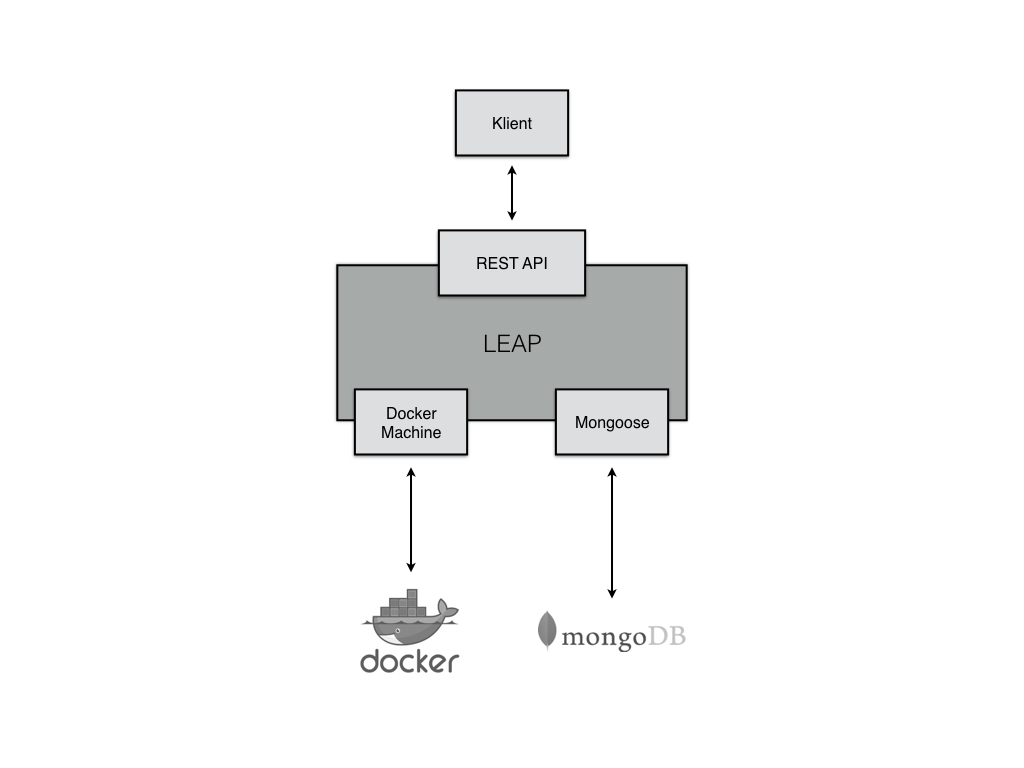
\includegraphics[scale=0.4]{leap_arch.eps}
\caption{Systemarkitektur för LEAP}
\label{fig:LeapArch}
\end{figure}

\newpage
\subsubsection{Uppladdning och inlämning}

När en lärare ska skapa en uppgift och ladda upp en tillhörande testfil hanteras detta av LEAP i följande steg: 
\begin{enumerate}
\item
Läraren loggar in i systemet och väljer att skapa en uppgift.
\item
Till uppgiften måste läraren bifoga testfall\footnote{Dessa testfall har en lärare skapat vid ett tidigare tillfälle} till uppgiften och ett program som testfallen kommer köras mot senare för att verifiera att testfallen är korrekta.
\item
Läraren får valmöjligheten att skapa ett tillhörande quiz till uppgiften.
\item
Läraren skickar en förfrågan om att skapa uppgiften.
\item
Servern tar emot förfrågan om att skapa en ny uppgift.
\item
Servern startar exekveringen av lärarens testfallen mot lärarens uppladdade program. Detta steg genomförs för att garantera att lärarens testfall går igenom mot den tänkta lösningen som är lärarens uppladdade program.
\item
Om exekvering av alla testfall passerades sparas uppgiften i databasen och ges då ett unikt ID. Detta ID skickas sedan tillbaka till läraren tillsammans med ett meddelande om att uppgiften har sparats i databasen. Om exekveringen av något testfall misslyckades skickar servern tillbaka ett svar till läraren om att uppladdningen misslyckades tillsammans med ett felmeddelande om vad som gick fel.
\end{enumerate}

\newpage

För att underlätta beskrivningen av hur LEAP hanterar en inlämning av en student valde vi att använda oss av ett aktivitetsdiagram. Figur \ref{fig:LeapFlow} nedanför visar flödet i LEAP när en student ska genomföra och lämna in en lösning till en uppgift.

\begin{figure}[ht!]
\centering
\includegraphics[scale=0.25]{correct_leap_flow.eps}
\caption{Aktivitetsdiagram över inlämningsprocessen för en student}
\label{fig:LeapFlow}
\end{figure}

Figuren visar hur genomförandet av en uppgift går till vilket kan involvera ett quiz beroende på lärarens val att lägga till en quiz eller ej. En uppgift kommer dock alltid att ha testfall som testar studentens program. När LEAP exekverar testfallen mot studentens program vid inlämning av en uppgift eller mot lärarens program vid uppladdning av en uppgift sker det i en Docker-container för att skydda servern mot eventuell skadlig kod.

\newpage

I Figur \ref{fig:leapTeknisk1} och Figur \ref{fig:leapTeknisk2} visualiseras det hur LEAP hanterar exekveringen av testfallen när en student skickar en lösning till en uppgift. Vi förutsätter att studenten redan har fullföljt uppgiftens eventuella quiz och att studenten har skickat en förfrågan med sin lösning och uppgiftens ID till servern via klienten. Varje gång en student skickar sin lösning till LEAP skapar servern en unik temporär mapp. Syftet med mappen är att hantera kommunikationen mellan servern och Docker-containern genom att servern delar den temporära mappen med Docker-containern. Kommunikationen sker genom att servern sparar studentens lösning och testfallen för uppgiften i mappen och på så sätt kan Docker-containern få tillgång till dessa och starta exekvering av testfallen mot studentens lösning. Exekveringens utdata sparas till en textfil och på så sätt kan servern få tillgång och tolka utdatan och därigenom avgöra om studenten har passerat alla testfall eller ej. Figur \ref{fig:leapTeknisk1} presenterar visuellt hur servern skapar den temporära mappen med tillhörande filer.

\begin{figure}[ht!]
\centering
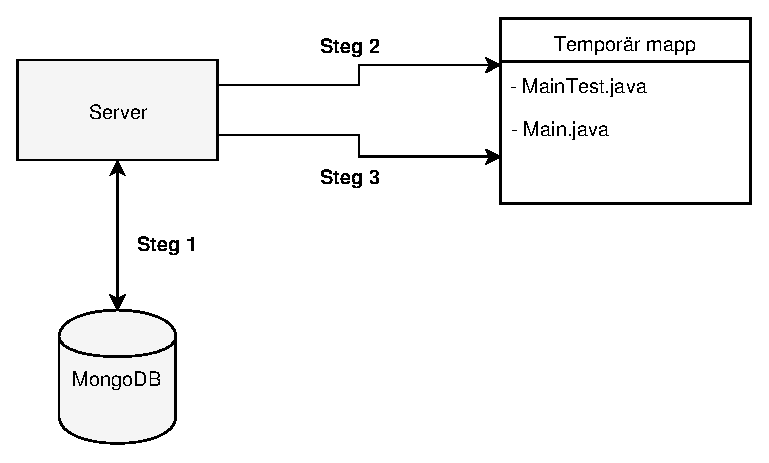
\includegraphics[scale=0.8]{leap_teknisk_1.eps}
\caption{Aktivitetsdiagram över inlämningsprocessen för en student}
\label{fig:leapTeknisk1}
\end{figure}

\begin{description}
    \item [Steg 1] Servern hämtar testfallen för uppgiften baserat på uppgiftens ID som serven fick genom studentens förfrågan.
    \item [Steg 2] Efter att servern har hämtat testfallen från databasen skapar servern den temporära mappen och skapar även filen \textit{MainTest.java} i den temporära mappen och sedan skriver servern testfallen till \textit{MainTest.java}
    \item [Steg 3] Efter steg 2, flyttar servern studentens lösning beståendes av en en kodfil till den temporära mappen och namnger studentens lösning, kodfil, till \textit{Main.java}
\end{description}

\newpage
Figur \ref{fig:leapTeknisk2} presenterar visuellt hur servern startar exekveringen av Docker-containern och hur servern får tillbaka utdatan från de exekverade testfallen som sker i Docker-containern.

\begin{figure}[ht!]
\centering
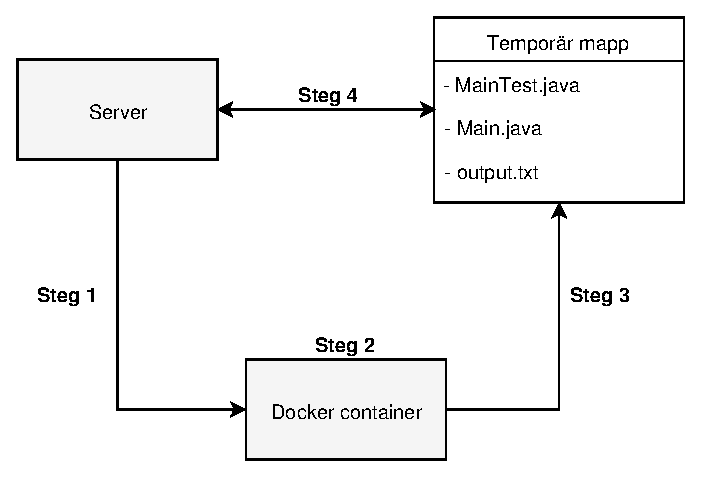
\includegraphics[scale=0.8]{leap_teknisk_2.eps}
\caption{Aktivitetsdiagram över inlämningsprocessen för en student}
\label{fig:leapTeknisk2}
\end{figure}

\begin{description}
    \item [Steg 1] Servern startar exekveringen av Docker-containern
    \item [Steg 2] När exekveringen av Docker-containern startas genom servern kör Docker-containern testfallen som finns i filen \textit{MainTest.java} mot kodfilen \textit{Main.java}. Dessa filer finns i den temporära mappen som servern delade Docker-containern.
    \item [Steg 3] När exekveringen av testfallen är klara skriver Docker-containern utdatan till en textfil med namnet \textit{output.txt} och placerar textfilen i den temporära mappen och på så sätt kan servern ta del av testfallens utdata.
    \item [Steg 4] Servern hämtar innehållet, testfallens utdata, i filen \textit{output.txt} och tolkar utdatan för att kunna avgöra om studentens lösning har passerat testfallen eller ej. Om samtliga testfall passerades meddelar servern studenten att lösningen godkändes. Om något testfall inte passerade meddelar servern studenten att lösningen ej godkändes och skickar även med utdatan från testfallen.
\end{description}

\newpage
\subsection{Kontrollerade experiment} \label{experiment}

Här presenteras resultaten från de kontrollerade experimenten som vi utförde på studenter vid Malmö Högskola. Vid de frågor som involverade att testpersonerna fick göra ställningstagande krävde vi att testpersonerna motiverade dessa. För att kunna tolka testpersonernas motiveringar och åsikter har vi identifierat värdeord i motiveringarna och åsikterna samt även identifierat vad värdeorden syftar på. Genom detta har vi kunnat gruppera testpersonernas åsikter och motiveringar och på så sätt kunnat sammanfatta och dra slutsatser från åsikterna och motiveringarna. 
\\
\\
I tabell \ref{tab:Testpersoner} ges en översikt över testpersonerna i form av ålder, kön och vilket program som de läser.

\begin{table}[h!]
	\centering
	\caption{Överblick av testpersonerna}
	\label{tab:Testpersoner}
	\begin{tabular}{c c c c c}
		\toprule
		Testperson & Ålder & Kön & Program & Termin\\
		\midrule
		1 & 26 & Man & Datavetenskap och applikationsutveckling & Andra\\
		2 & 28 & Man & Systemutvecklare & Sjätte\\
		3 & 32 & Kvinna & Systemutvecklare & Fjärde\\
		4 & 22 & Man & Informationsarkitekt & Sjätte\\
		5 & 23 & Man & Systemutvecklare & Sjätte\\
		6 & 23 & Man & Systemutvecklare & Fjärde\\
		7 & 39 & Kvinna & Systemutvecklare & Sjätte\\
		8 & 39 & Man & Spelutveckling & Fjärde\\
		\bottomrule
	\end{tabular}
\end{table}
Av åtta testpersonerna är två kvinnor och fem av testpersonerna läser till Systemutvecklare vid Malmö Högskola.

\subsubsection{Användarupplevelse}\label{Användarupplevelse}
Efter att testpersonerna utfört användartestet fick de ge sina synpunkter på användarupplevelsen. I figur \ref{fig:GeneralUX} presenteras resultatet på frågan \textit{Hur skulle du bedöma den allmänna användarupplevelsen (UX) av vår prototyp?}, där 1 motsvarar väldigt dåligt och 7 motsvarar mycket bra.

\begin{figure}[ht!]
\centering
\includegraphics[scale=0.6]{general_UX2.eps}
\caption{Allmänna användarupplevelsen av prototypen}
\label{fig:GeneralUX2}
\end{figure}

Testpersonernas åsikter var delade när det kommer till detaljrikedomen i återkopplingen. Tre personer upplevde att återkopplingen tydligt visar vad felet i programmet är. Dock upplevde tre personer att återkopplingen som vår prototyp gav var svårtydlig och svårförstådd. Merparten av testpersonerna upplevde att vår prototyp var enkel att använda eftersom navigeringen var tydlig och att det var tydligt hur man skickade in en uppgift för bedömning. 
Vi hade även en fråga där vi ville att testpersonerna skulle föreslå förbättringar för vår prototyp. Där nämner samtliga att återkopplingen kan bli bättre på olika sätt. De nämner dels att den kan bli tydligare och mer strukturerad för att det ska vara lättare att veta vad felet i programmet är men även att det hade varit bra att få tips eller exempel på hur felen kan lösas. 

Vi ställde även en fråga om testpersonerna tror att det skulle vara användbart att använda vår prototyp vid programmeringskurser. Samtliga studenter ställer sig positiva, det vill säga de svarade ja, till att använda vår prototyp vid programmeringskurser. Merparten av testpersonerna menar att direkt återkoppling är anledningen till att de anser att vår prototyp kan användas vid programmeringskurser. En av testpersonerna anser dock att återkopplingen som ges från en lärare eller en labbhandledare är mer givande. Två av testpersonerna påpekar att med vår prototyp skulle studenterna bli mer självständiga. En av dem menar att vid laborationer finns det inte alltid utrymme att få sina uppgifter bedömda eftersom antalet studenter är markant fler än antalet lärare och labbhandledare. Vidare menar testpersonen att det finns få redovisningstider vilket medför att studenter har svårt att få sina uppgifter redovisade och bedömda samt att stressen för lärare att bedöma uppgifterna minskar med användningen av vår prototyp.

\subsubsection{Återkoppling}\label{Återkoppling}

Vi ställde även frågor till testpersonerna om hur de upplevde att få direkt återkoppling och hur de upplevde detaljrikedomen i återkopplingen. Vi frågade testpersonerna hur de upplevde att få direkt återkoppling på en skala från ett till sju, där 1 är väldigt dåligt och 7 motsvarar mycket bra.
Samtliga testpersoner svarade med en 7:a. De påpekade att det var skönt att slippa vänta på att få en uppgift bedömd eftersom testpersonerna tycker att återkoppling ska ges när de är inne i tänket för uppgiften. En av testpersonerna svarar att det är ineffektivt med bedömning som involverar en lärare när det gäller direkt återkoppling eftersom det kan dröja upp till två veckor innan en uppgift blir bedömd. En annan testperson svarar även att med direkt återkoppling kan missuppfattningar kring en uppgift upptäckas tidigare jämfört med bedömning som involverar en lärare. En av testpersonerna svarar även att uppgifter kan bli enklare vid direkt återkoppling, men att det kan lösas genom att sätta en begränsning på antalet inlämningar.

Testpersonerna fick även besvara frågan \textit{Hur upplevde du detaljrikedomen i återkopplingen?}, där 1 motsvarar väldigt dålig och 7 motsvarar mycket bra. Svaren presenteras i figur \ref{fig:DetailFeedback}.

\begin{figure}[ht!]
\centering
\includegraphics[scale=0.6]{detail_feedback2.eps}
\caption{Upplevelsen av detaljrikedomen i återkopplingen}
\label{fig:DetailFeedback}
\end{figure}

Sju av testpersoner upplevde att detaljrikedomen i återkopplingen var hög men vissa menar att återkopplingen var svårtolkad och kunde presenterats och strukturerats på ett enklare och mer konkret sätt. En av testpersonerna menar att prototypens återkoppling inte är lika givande jämfört med återkopplingen från en lärare eftersom en lärare även kan ge en förklaring på varför felet uppstod. De menar även att det kan vara bra att ge tips eller exempel för att lösa felen.

\newpage
\subsubsection{Quiz}

Eftersom vår prototyp även gör det möjligt att använda ett quiz vid uppgifterna, ställde vi frågor relaterat till quizzet. I figur \ref{fig:QuizHelps} visas resultatet på frågan \textit{Hur mycket tror du att ett quiz hjälper studenter i deras programmeringsutveckling och förståelse?}, där 1 motsvarar inte alls och 7 väldigt mycket.

\begin{figure}[ht!]
\centering
\includegraphics[scale=0.6]{quiz_helps2.eps}
\caption{Betydelsen av quiz för utvecklingen}
\label{fig:QuizHelps}
\end{figure}

Sju av testpersonerna ställer sig positiva till att använda quiz för att förbättra studenternas förståelse och kunskap. Det är en testperson som ställer sig negativt till detta. Testpersonen tror inte att det hjälper studenterna med ett quiz utan menar istället att det är bättre med praktiska moment som programmeringsuppgifter eller laborationer för att utveckla studenternas förståelse och kunskaper. Personen menar att användningen av quiz istället är till mest nytta för läraren då läraren kan få en bättre bild av studenternas faktiska förståelse.

Två av personerna menar att det är viktigt med teori och begrepp för att förstå helheten och att det utan viss förståelse är svårt att programmera eller ha förståelse för varför lösningen ser ut som den gör.

Vidare ställde vi frågan \textit{När tycker du att ett quiz bör användas?} där testpersonerna kunde välja mellan (1) \textit{Innan programmeringsuppgift} (2) \textit{Efter programmeringsuppgift} (3) \textit{Både och} (4) \textit{Inte alls}. Resultatet från frågan var att fyra testpersoner svarade (1) och de andra fyra svarade (3). De personer som tyckte att ett quiz bör användas innan  programmeringsuppgiften menar att det kommer hjälpa studenten att genomföra programmeringsuppgiften eftersom det kräver att studenten har en viss grad av förståelse innan programmeringen påbörjas. De påpekar även att ett quiz hjälper studenterna att inse inom vilka områden de behöver förbättra sin förståelse. 

De personer som tyckte att ett quiz bör användas både innan och efter programmeringsuppgiften har liknande åsikter om varför de anser att det ska vara innan. Anledningen till att de anser att ett quiz även borde finnas efter en programmeringsuppgift är för att verifiera att studenten har erhållit de förväntade kunskaperna från programmeringsuppgiften. 

\subsubsection{Traditionellt eller automatiserat?}

För att kunna jämföra traditionell och automatiserad bedömning ställde vi frågor till testpersonerna där de fick lyfta fram fördelar och nackdelar om respektive sätt följt av att de fick göra en bedömning av vilket sätt de tror är bäst för deras utveckling som programmerare.

Fördelar med automatiserade bedömningssystem som testpersonerna lyfte fram är liknande de delar som beskrivits under avsnitt \ref{Återkoppling} och \ref{Användarupplevelse} som snabbare återkoppling och att studenterna blir mer självständiga. En av testpersonerna påpekade att de studenter som har problem kan få mer hjälp av lärare och labbhandledare eftersom de andra studenterna blir mer självständiga och kräver därav inte lika mycket av lärarens resurser. Testpersonen menar även att med ett automatiserat bedömningssystem kan uppgifterna bli bättre genom åren eftersom ett sådant system kan användas av flera högskolor och på så sätt kan de olika högskolorna samarbeta för att göra uppgifterna bättre för studenterna. En av testpersonerna menar även att med automatiserade bedömningssystem kan studenter rätta sina egna fel och undviker därmed att skämmas över sina inskickade program eller kodfiler som de inte är nöjda med.

Nackdelar som testpersonerna lyfte fram med automatiserade bedömningssystem är att återkopplingen kan vara svårtolkad, vilket testpersonerna har nämnt vid tidigare tillfällen. Två av testpersonerna menar att det är svårt att verifiera kodkvalitén i studenternas program. En av dem menar att ett problem går att lösa på många olika sätt och där vissa är bättre än andra. De menar även att det är svårare för ett bedömningssystem än för en lärare eller labbhandledare att ge förslag på förbättringar som studenterna kan göra i sina program vilket exempelvis kan förbättra läsbarheten och effektiviteten. En person påpekar att lärare kan frestas av att konstruera uppgifter av enklare karaktär då det medför enklare testning.

Tre av testpersonerna ansåg att det inte finns några fördelar med att använda ett traditionellt bedömningssätt som involverar en lärare. De andra testpersonerna menar att med en lärare eller en labbhandledare kan en mer kvalitativ återkoppling ges. En av testpersonerna menar att en student då kan få svar på varför något är fel i deras kod istället för vad som är fel. En annan testperson påpekar att läraren kan granska programmet utifrån ett läsbarhetsperspektiv vilket inte ett bedömningssystem kan göra.

Nackdelar som testpersonerna lyfter fram med traditionell bedömning är att det dels är tidskrävande för lärare och labbhandledare men och dels att det tar tid för studenterna att få återkoppling och bedömning. En av testpersonerna menar att bara för att det är en lärare som bedömer en uppgift behöver inte det automatiskt betyda att återkopplingen kommer hjälpa studenten att genomföra uppgiften. Vidare menar testpersonen att återkopplingen från en lärare ibland enbart uppger att studenten inte klarat uppgiften och att återkopplingen saknar motivering till varför studenten inte klarat uppgiften. En annan testperson är inne på samma spår, där testpersonen menar att de krävs att det finns bra labbhandledare som kan ge korrekt återkoppling, vilket enligt testpersonen inte alltid är fallet.

Vi avslutade med att ställa frågan \textit{Vilket av traditionellt och automatiserat sätt tror du är bäst för din utveckling som programmerare att använda vid programmeringskurser?}. Resultatet på denna fråga presenteras i figur \ref{fig:TradvsAuto}.

\begin{figure}[ht!]
\centering
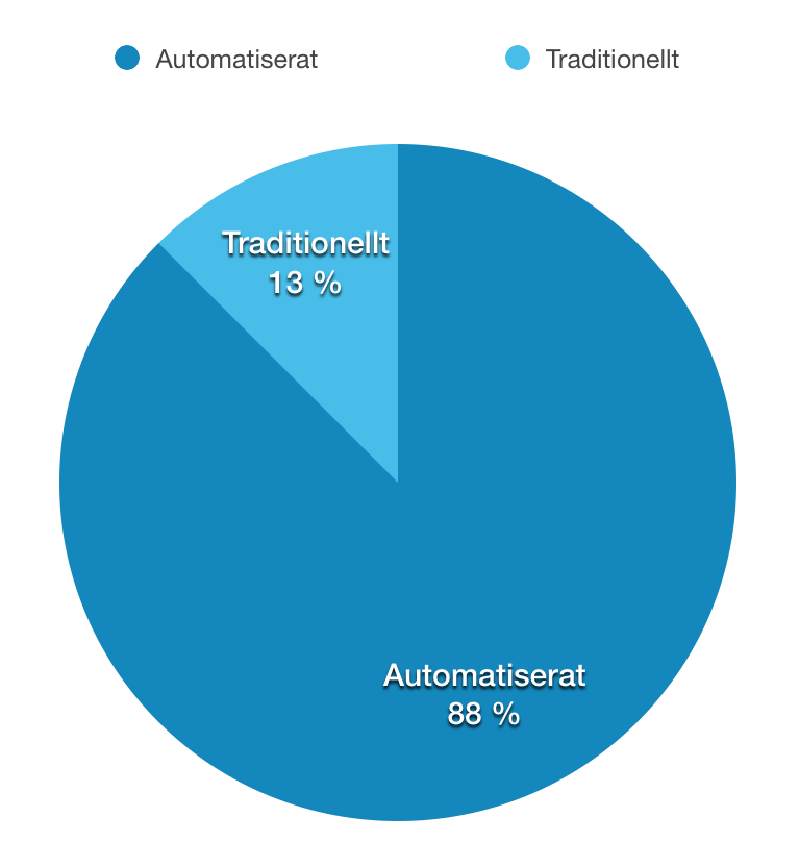
\includegraphics[scale=0.5]{trad_vs_auto.eps}
\caption{Traditionellt eller automatiserat}
\label{fig:TradvsAuto}
\end{figure}

Det är sju av åtta testpersoner som anser att automatiserad bedömning är bättre för deras utveckling som programmerare. Motivering till deras val är fördelarna som nämnts ovanför som snabbare återkoppling och ökad självständighet för studenterna. En testperson menar att ett automatiskt bedömningssystem inte behöver utesluta en labbhandledare eller lärare helt utan mer fungera som ett stöd till dessa. En annan testperson menar att automatiskt och traditionellt bedömningssätt uppfyller olika syften. Testpersonen menar att ett traditionellt bedömningssätt är bättre vid introduktionskurser eftersom det kan krävas mer hjälp och bättre återkoppling. Vidare menar testpersonen att ett automatiserat system är mer lämpligt att använda i kurser med avancerat innehåll eftersom fokus i dessa kurser är problemlösning av specifika problem istället för utlärning inom ett specifikt ämne vilket är fokus i introduktionskurser.

\newpage
\section{Analys och diskussion}

I en studie av Carter m. fl. \cite{carter} framkom det att åsikterna om bedömningssystem bland de intervjuade lärarna i studien var mer positiv ju mer erfarenhet av bedömningssystem de hade. De lärare utan tidigare erfarenhet av bedömningssystem ansåg att sådana system ej var lämpliga för att testa studenters kunskaper och att kvalitén på återkopplingen var låg. Detta resultat kan jämföras med resultatet från de intervjuer som vi genomförde med tre lärare på Malmö Högskola eftersom två av lärarna inte trodde på att använda automatiserade bedömningssystem vid programmeringskurser och att dessa två lärare aldrig tidigare använt ett bedömningssystem i deras programmeringskurser. Därför tror vi att deras negativa åsikter kan bero på deras oerfarenhet av bedömningssystem. Och det är just lärarna som avgör hur bra ett bedömningssystem är eftersom det är upp till lärarna att utforma uppgifterna och ta fram välgenomtänkta och heltäckande testfall. Utformningen av uppgifter och tillhörande testfall har i tidigare studier identifierats som framgångsfaktorer för ett bedömningssystem []. Detta eftersom vid automatiserad bedömning krävs det att uppgifters krav är mer precisa än vid manuell bedömning för att undvika tvetydigheter särskilt när det handlar om indata och utdata []. När det kommer till testfall är det viktigt att de är genomtänkta och heltäckande för att förhindra att felaktiga programmeringslösningar godkänns []. Men nackdelen med dessa framgångsfaktorer är att de kan kräva mer resurser än vad som krävs vid manuell bedömning särskilt om antalet studenter är hanterligt manuellt. Tidigare studier \cite{ala-mutka} \cite{cinelli} menar att utformningen av uppgifter och testfall för automatiserade bedömningssytem kräver mer resurser än utformningen av uppgifter som bedöms manuellt. Men trots att utformningen av uppgifter och testfall för automatiserad bedömning kräver mer resurser hjälper automatiserad bedömningssystem lärare att minska deras arbetsbelastning som läggs på att manuellt verifiera att studenternas programmeringslösning är korrekta \cite{enstrom}.
\\
\\
Att verifiera lösningens korrekthet är en funktionalitetsbedömning, vilket är den typ av bedömning som LEAP genomför av studenternas lösning. En fördel med att automatisera funktionalitetsbedömningen är att ett bedömningssystem inte kommer godkänna en lösning förrän alla testfall passeras och om testfallen är väl genomtänkta och heltäckande är det lättare att garantera lösningens korrekthet än vid manuell bedömning. Därmed anser vi att ett bedömningssystem utför funktionalitetsbedömning snabbare och utförligare än vad en lärare gör.
\\
\\
Men när det kommer till bedömning av mer kvalitativa aspekter tror vi att bedömningen av en lärare är att föredra, vilket stöds av flertalet andra studier [KÄLLOR] men även av resultaten från de kontrollerade experimenten. Testpersonerna menar dels att lärare kan bedöma aspekter som kodkvalité, läsbarhet och även att en lärare kan ge förbättringsförslag samt best practices vilket är betydligt svårare för ett bedömningssystem. Däremot är det inte säkert att studenter får kvalitativ återkoppling enbart för att återkopplingen ges av lärare, vilket lyftes fram av en testperson från de kontrollerade experimenten. En annan nackdel med manuell bedömning är risken för subjektiv bedömning större än vad den är vid automatiserade bedömningssystem. En av testpersonerna ansåg att ett bedömningssystem inte lämpar sig att användas vid introduktionskurser utan att det istället borde användas vid mer avancerade kurser eftersom fokus i dessa kurser är problemlösning av specifika problem istället för utlärning inom ett specifikt ämne vilket är fokus i introduktionskurser. Detta stöds av Ahoniemi and Reinikainen som menar att oerfarna studenter kräver grundlig och personlig återkoppling på deras programmeringsuppgifter för att de ska lära sig av sina misstag och på så sätt kunna förbättra sina kunskaper. Däremot visar studien [Law, Lee, Yu] hur ett bedömningssystem uppmuntrade och motiverade studenters vilja att lära sig. Men trots att studien visar att de blir mer motiverade är fortfarande manuell bedömning att föredra framför automatisk bedömning när bedömningen behandlar kvalitativa aspekter, vilket har bevisats i flertalet andra studier [].
\\
\\
En annan fördel med automatiserade bedömningssystem är att studenter, särskilt de bättre studenterna, blir mer självständiga eftersom ett bedömningssystem har möjligheten att vara tillgängligt dygnet runt. Som en av testpersonerna lyfte fram kan de studenter som har lättare för en del moment kräva mindre tid av en lärare eller labbassistent för att få deras uppgifter bedömda vilket gör att en lärare eller labbassistent har mer tid över till de som behöver mer personlig och grundlig återkoppling och hjälp.
\\
\\
Utifrån våra resultat är det svårt att avgöra hur ett bedömningssystem av den här typen har för påverkan på studenters programmeringskunskaper. Vi tror att det skulle krävas en studie som under en längre period analyserade effekterna av att använda ett bedömningssystem av den här typen i en programmeringskurs för att kunna avgöra om studenters programmeringskunskaper förbättras. I en studie av Daly och Horgan \cite{roboprof_4} analyserade de under ett år effekterna av att använda det system författarna utvecklat, RoboProf, i en programmeringskurs för Java-programmering. Totalt ingick 300 studenter i studien och resultaten visar att de studenter som gjorde de uppgifter som fanns till RoboProf presterade signifikant mycket bättre än de studenter som inte gjorde det. Liknande resultat har även presenterats i andra studier \cite{higgins_coursemarker_12} \cite{japanerna_1}. Resultaten från de kontrollerade experimenten visar att de studenter som ingick i studien har en positiv syn på användningen av ett bedömningssystem av den här typen i programmeringskurser och vår förhoppning är att användningen av LEAP i en programmeringskurs ska leda till resultat som visar att LEAP ökar studenters programmeringskunskaper i högre grad än enbart traditionell bedömning. 
\\
\\
En av testpersonerna i de kontrollerade experimenten påpekar att en möjlig negativ aspekt av användningen av automatiska bedömningssystem är att studenters utrymme för kreativitet i sina lösningar hämmas. Eftersom kraven för uppgifter som ska bedömas av ett automatiskt bedömningssystem måste vara mycket precisa och väldefinierade kan det leda till att lärare utformar uppgifter på ett sätt som gör det svårt för studenten att utnyttja sin fulla kreativitet i sin lösning \cite{pieterse}. Vi tycker av dessa skäl att uppgifter av mindre omfattning där design och struktur inte har någon påverkan på lösningens kvalité bör lämpa sig bra för bedömning av ett automatiskt bedömningssystem medans större uppgifter kan kräva en viss grad av manuell bedömning. Ett exempel på en uppgift av mindre omfattning är att implementera en funktion som itererar genom en vektor och utför en validering för att sortera ut element från vektorn. En sådan uppgift är väldigt svår att bedöma avseende design till skillnad från en uppgift där studenten ska skapa en applikation som fungerar som ett adressregister vilket kan designas och implementeras på en mängd olika vis och som sätter studentens kreativitet på prov. Vi tror även att bedömningssystem lämpar sig att användas vid kurser som involverar algoritmer eftersom det då är möjligt att automatiskt testa om en algoritm har implementerats korrekt baserat på särskild indata.
\\
\\
Direkt återkoppling till studenterna är enligt resultatet från de kontrollerade experimenten den största fördelen med ett bedömningssystem dock upplevde testpersonerna att nackdelarna med återkopplingen från ett bedömningssystem kan vara att den är svårförstådd och att återkopplingen från en lärare är mer givande eftersom en lärare kan förklara varför felet uppstod och även ge mer kvalitativ återkoppling kring studentens lösning. Detta är något som stöds av Ala-Mutka \cite{ala-mutka}. De intervjuade lärarna är inne i samma tänk som testpersonerna från de kontrollerade experimenten då lärarna menar att deras återkoppling är mer givande för studenter och återkoppling är en viktig del i studenternas utveckling vilket stöds av Carless [Carless]. Carless menar att återkoppling är den viktigaste aspekten för en kvalitativ utveckling hos studenterna. Ala-Mutka \cite{ala-mutka} menar att trots att lärarens återkoppling kan vara av mer kvalitativ karaktär kompenseras kvalitén mot snabb återkoppling och tillgängligheten som ett bedömningssystem erbjuder. Carter m. fl. \cite{carter} presenterar från sin studie att en respondent från deras studie menar att direkt återkoppling med sämre kvalité är att föredra gentemot detaljerad och kvalitativ återkoppling som ges veckor senare. Vårt resultat från de kontrollerade experimenten stödjer påståendet eftersom sju av de åtta testpersonerna skulle föredra att använda ett automatiserat bedömningssystem istället för traditionell bedömning och direkt återkoppling var enligt testpersonerna den avgörande faktorn.
\\
\\
Vid intervjuerna med de tre lärarna vid Malmö Högskola framkom det att de efterfrågade möjligheten att använda quiz för att bedöma studenternas förståelse. Vi valde därför att i LEAP implementera möjligheten att använda ett quiz som en student måste avklara innan studenten kan lämna in sin lösning till programmeringsuppgiften. Resultaten från de kontrollerade experimenten visar att testpersonerna är övervägande positiva till att använda quiz för att förbättra studenternas förståelse och kunskaper. Vi tror att användningen av quiz får studenterna att på egen hand lära sig den bakomliggande teorin som är nödvändig för att sedan klara av att lösa programmeringsuppgiften och att ett quiz kan säkerställa att studenterna faktiskt har uppnått tillräcklig förståelse vilket var en av de punkter som de intervjuade lärarna ansåg var viktigast och som de ansåg att ett bedömningssystem inte kan bedöma. Vi tror även att med quiz får studenterna en ökad förståelse för programmering vilket därmed hjälper studenterna att nå högre betyg. I en studie av Woit och Mason \cite{woit_2003} genomförde de under fem år en kurs där upplägget på kursen varierade varje år. Under det året då de använde quiz som en del av kursens moment fann de en korrelation mellan resultaten på quiz och resultatet på den sista tentamina i slutet på kursen. Resultatet visar att varje student fick ungefär ett betyg högre än de studenter från de resterande åren.  
\\
\\
De tankar och åsikter vi fört fram i detta avsnitt bygger på resultaten från de intervjuer och kontrollerade experiment som genomförts. Det går att diskutera kring validiteten i resultaten eftersom antalet personer som ingick i intervjuerna och de kontrollerade experimenten är relativt få. Det som dock talar för resultatens validitet är att personerna som ingick i de två momenten enligt oss är väldigt representativa för respektive tänkta målgrupp. De tre intervjuade lärarna har alla lång dokumenterad erfarenhet inom utlärning av programmering till studenter och de studenter som ingick i de kontrollerade experimenten har olika bakgrund, utbildningar, ålder och kön.

%Fördelar
%- snabb återkoppling √
%- objektiv bedömning √
%- tillgänglighet, mer självständighet √
%- verifiera funktionaliteten bättre än en lärare, kan kolla HELA programmet vilket tar för mycket tid manuellt √
%- quiz som kan testa studenternas förståelse, bra källor på det. √
%- en viss säkerhet, körs åtminstone inte på lärarens dator

%Nackdelar
%- Tar tid att utforma testfall och uppgifter √
%- Svårt att verifiera kvalité i programmen √
%- Personlig feedback är mer kvalitativ, kan förklara vad felen beror på, men beror på hur bra handledaren är? √
%- Kreativitet hämmas √


\newpage
\section{Slutsatser}

\newpage
\section{Vidare forskning}


%
% Do not change
\newpage
\addcontentsline{toc}{section}{Referenser}

\bibliographystyle{ieeetr}
\bibliography{referenser}

\newpage

% Före Enkät
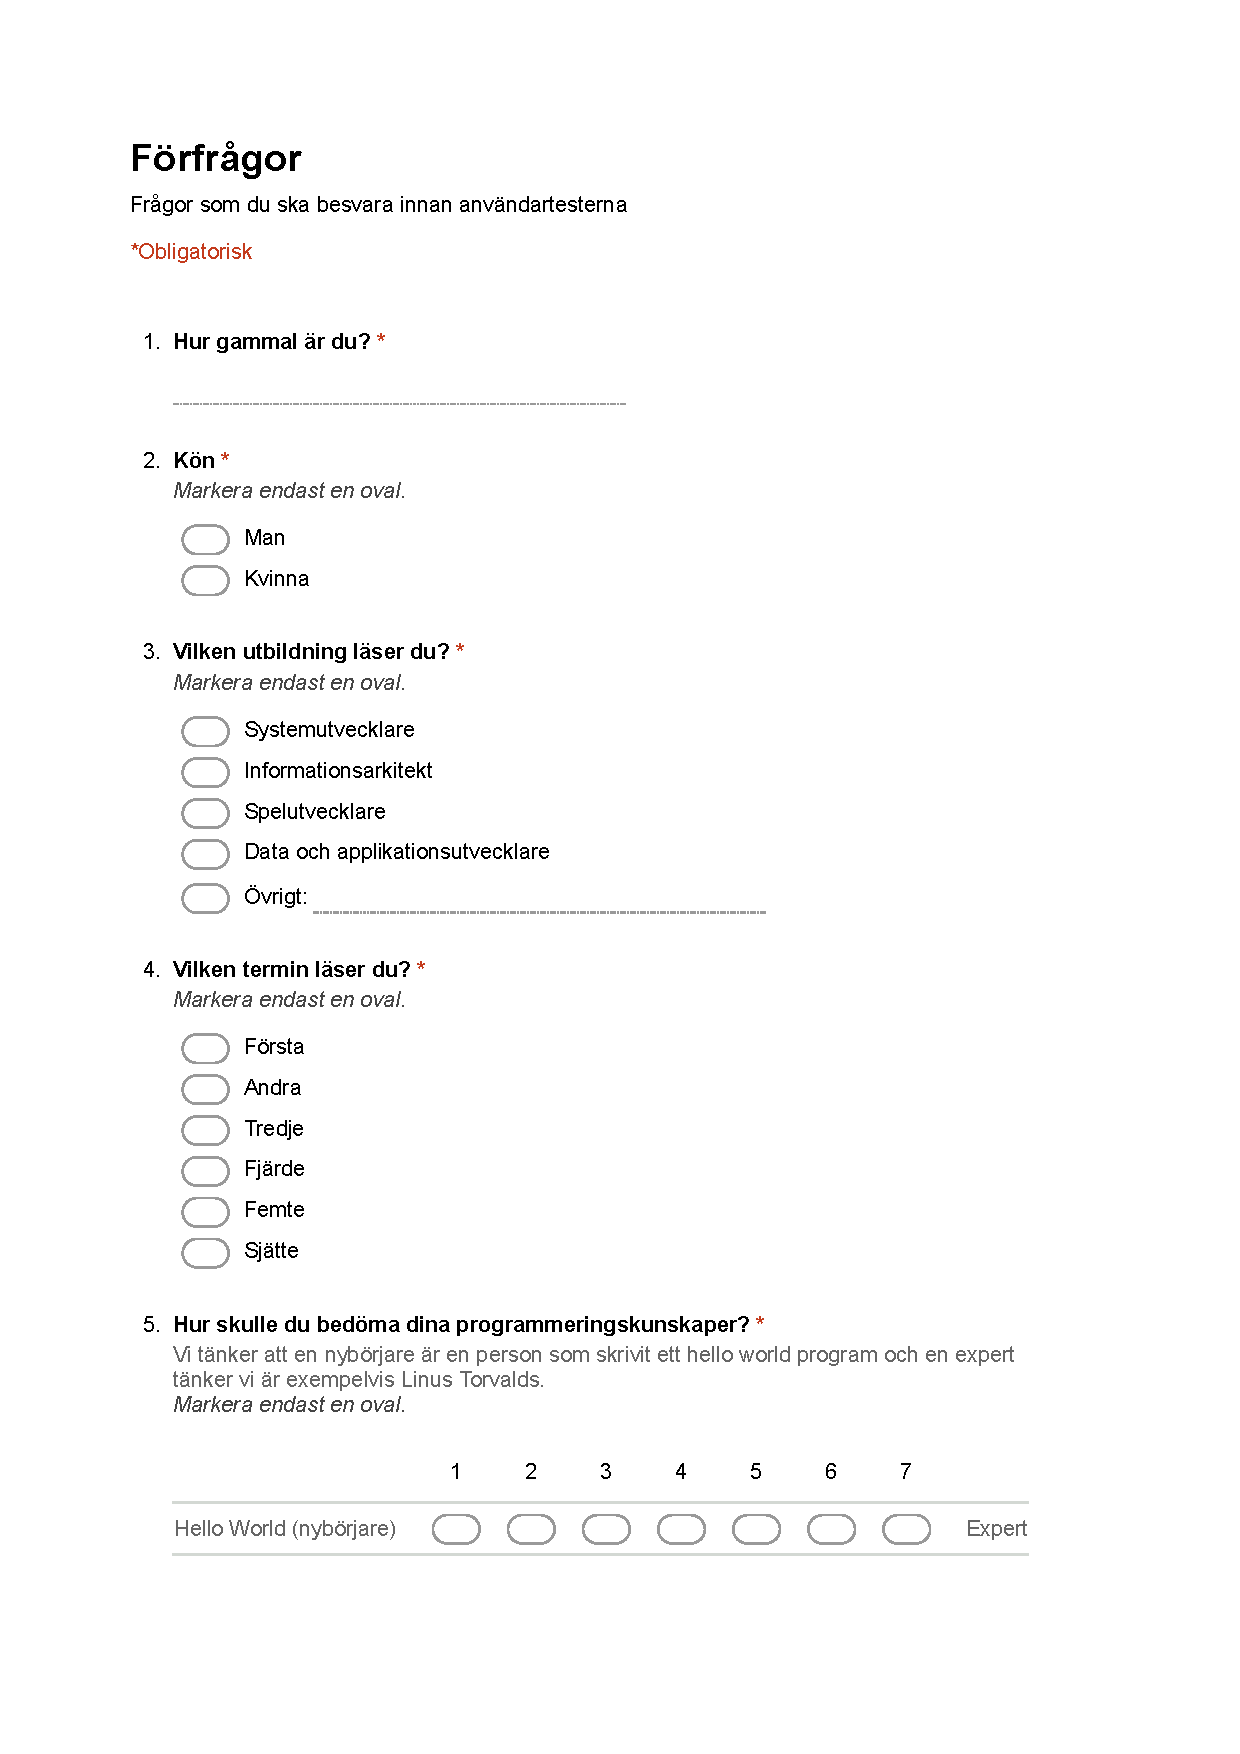
\includepdf[pages=1,scale=0.7,pagecommand=\section*{Appendix A}]{enkat_fore.pdf}
\includepdf[pages=2-,scale=0.7,pagecommand={}]{enkat_fore.pdf}

% Efter Enkät
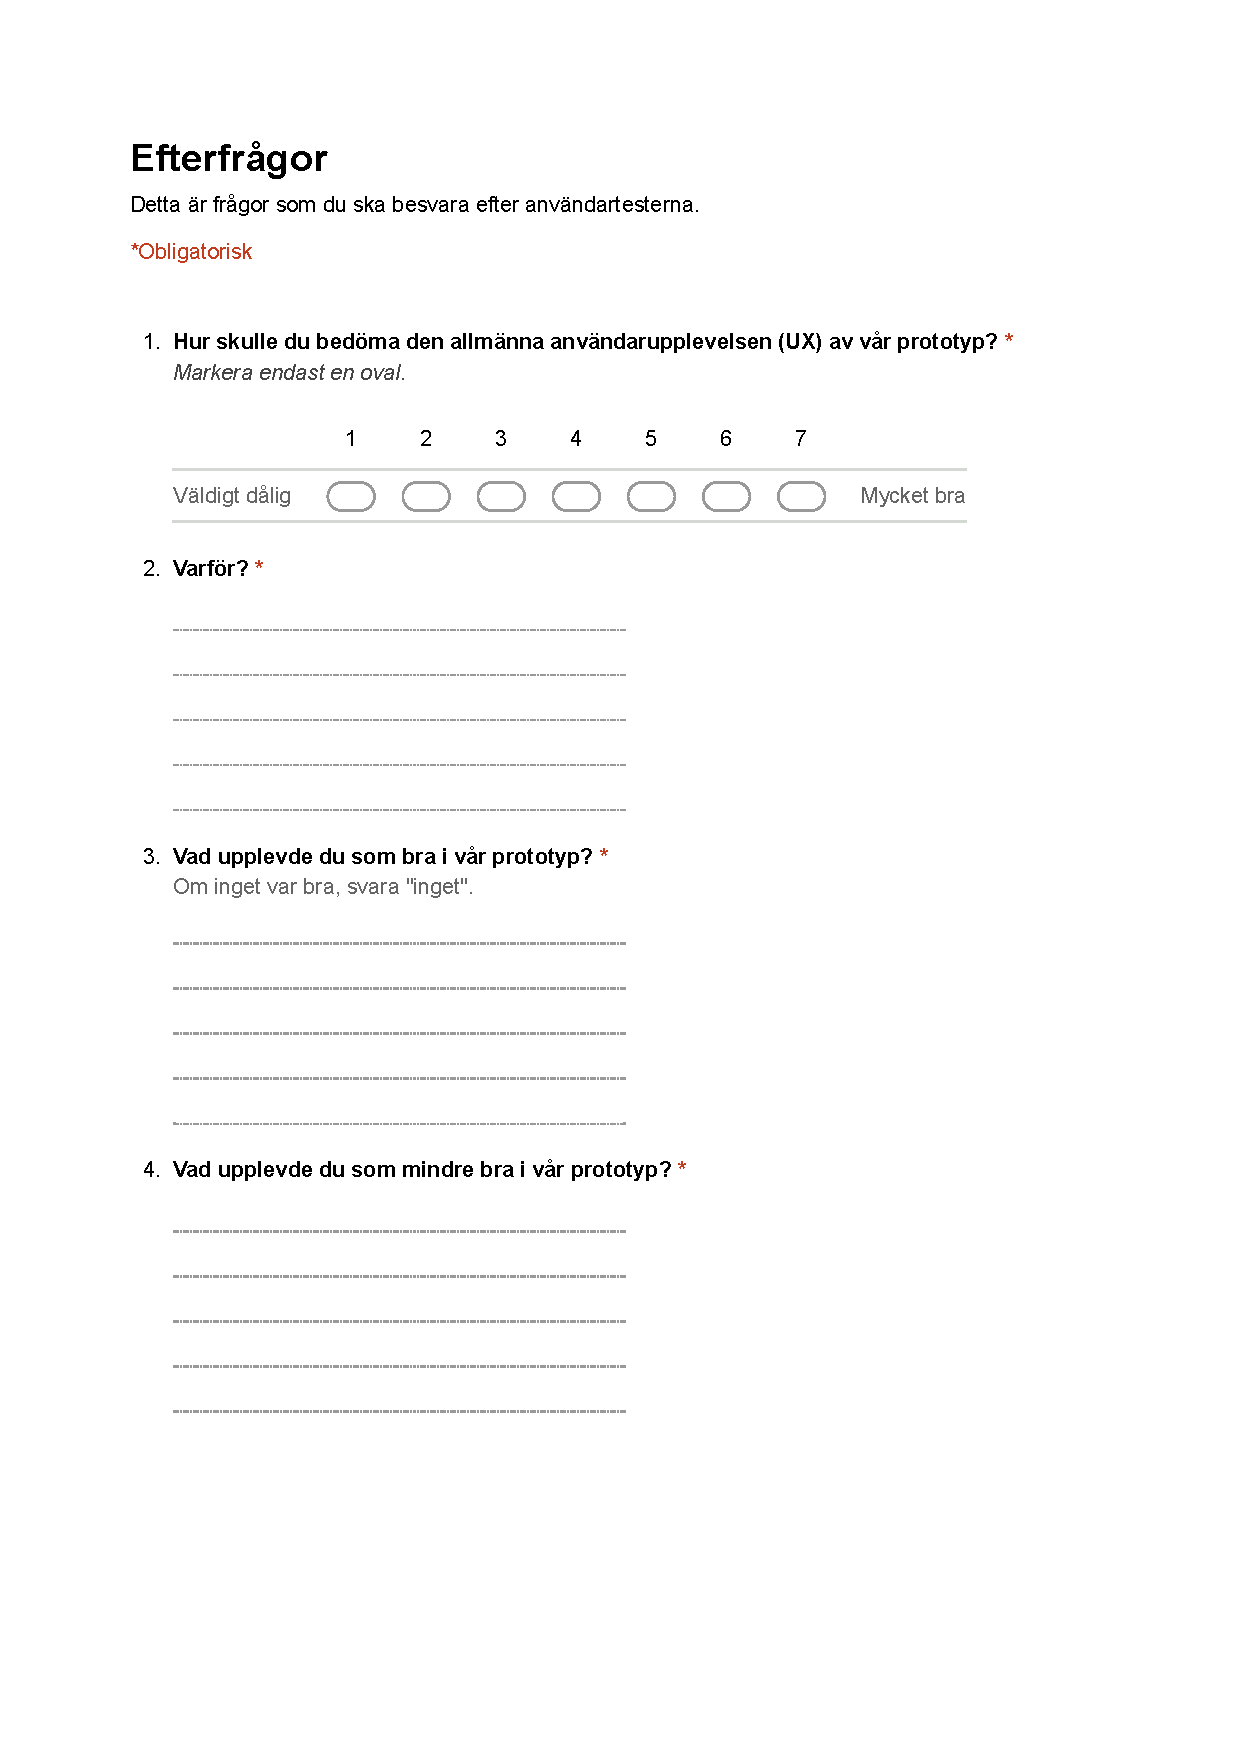
\includepdf[pages=1,scale=0.7,pagecommand=\section*{Appendix B}]{enkat_efter.pdf}
\includepdf[pages=2-,scale=0.7,pagecommand={}]{enkat_efter.pdf}

% Intervjufrågor
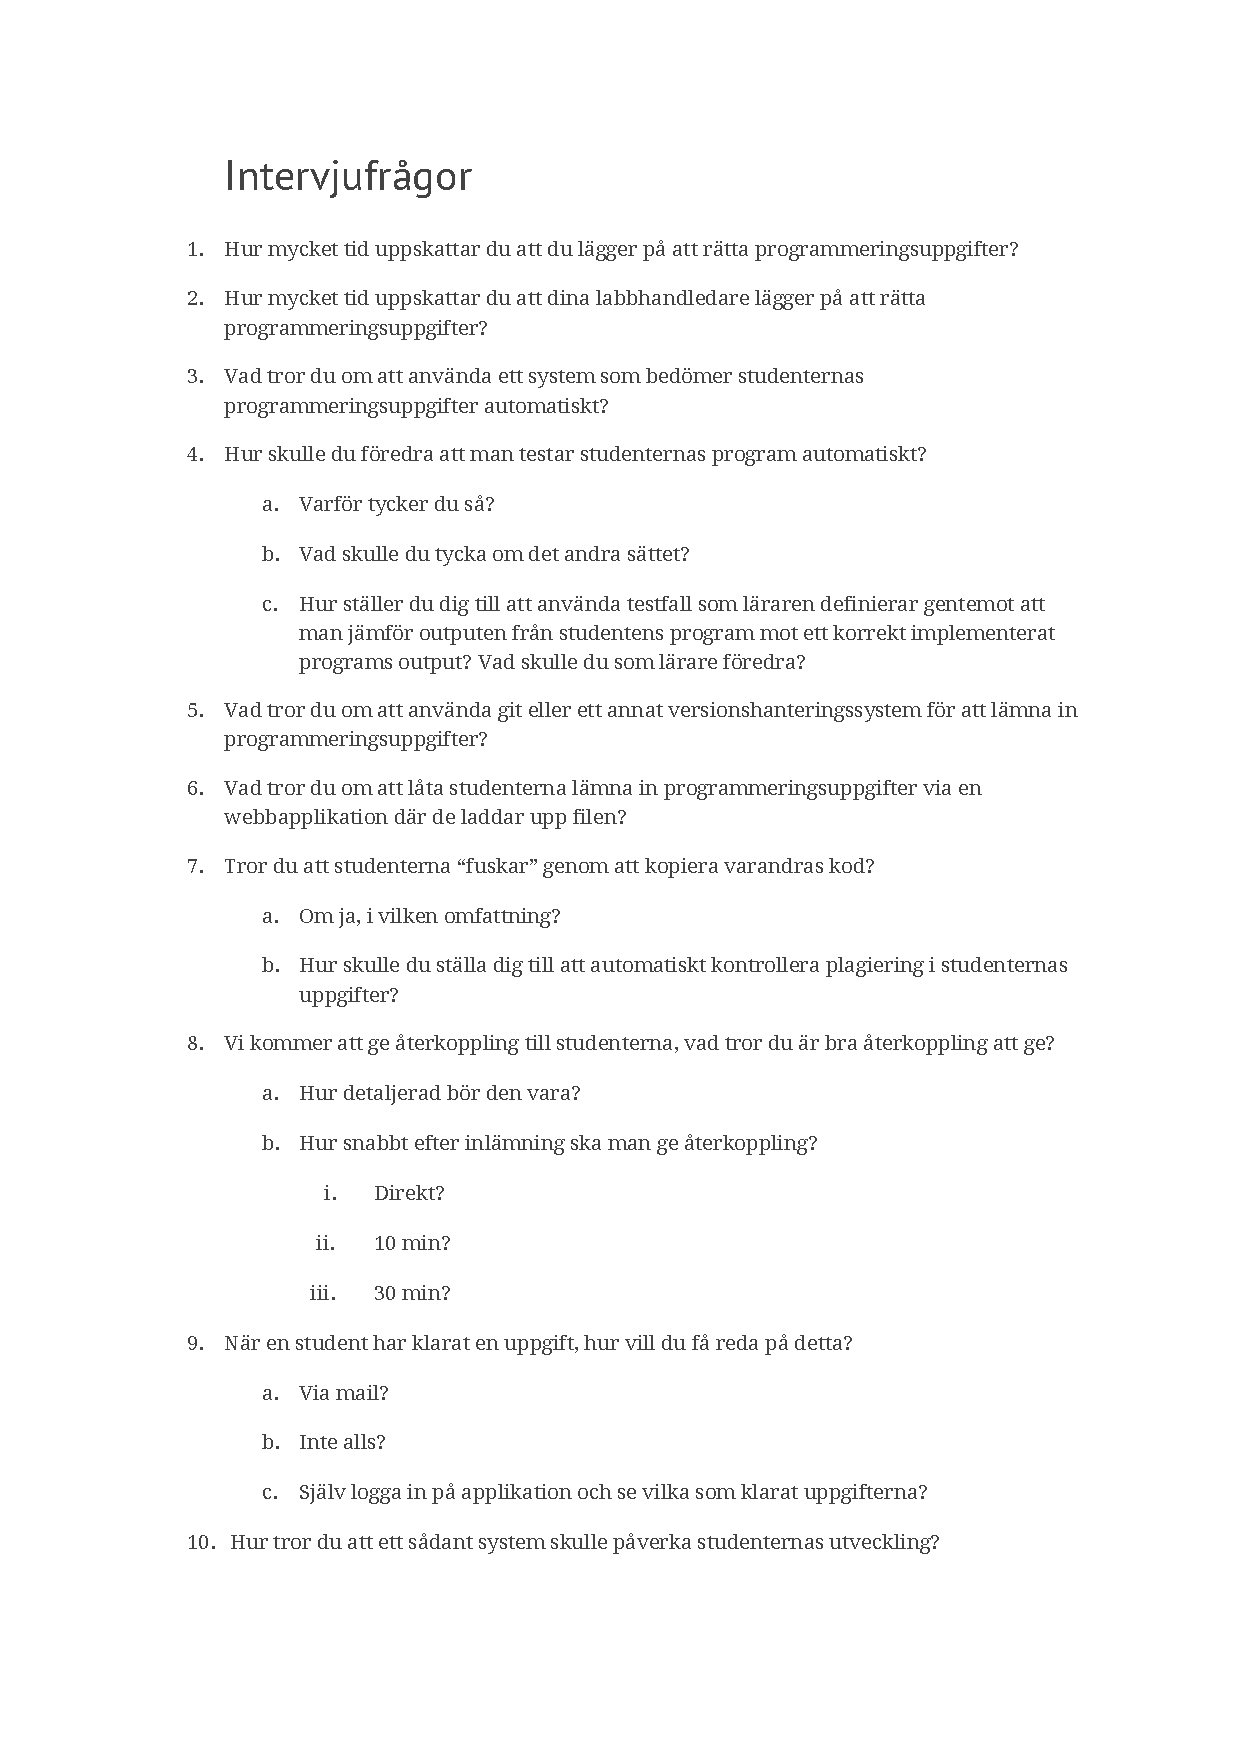
\includepdf[pages=1,scale=0.7,pagecommand=\section*{Appendix C}]{intervjufragor.pdf}


\end{document}